\documentclass[12pt, letterpaper]{article}
\usepackage[titletoc,title]{appendix}
\usepackage{color}
\usepackage{booktabs}
\usepackage[usenames,dvipsnames,svgnames,table]{xcolor}
\definecolor{dark-red}{rgb}{0.75,0.10,0.10}
\definecolor{bluish}{rgb}{0.05,0.05,0.85}

\usepackage[margin=1in]{geometry}
\usepackage[linkcolor=blue,
			colorlinks=true,
			urlcolor=blue,
			pdfstartview={XYZ null null 1.00},
			pdfpagemode=UseNone,
			citecolor={bluish},
			pdftitle={partisan_gap}]{hyperref}

\usepackage[resetlabels,labeled]{multibib}
\newcites{SI}{SI References}
\usepackage{natbib}

\usepackage{float}

\usepackage{geometry} % see geometry.pdf on how to lay out the page. There's lots.
\geometry{letterpaper}               % This is 8.5x11 paper. Options are a4paper or a5paper or other... 
\usepackage{graphicx}                % Handles inclusion of major graphics formats and allows use of 
\usepackage{amsfonts,amssymb,amsbsy}
\usepackage{amsxtra}
\usepackage{verbatim}
\setcitestyle{round,semicolon,aysep={},yysep={;}}
\usepackage{setspace}		     % Permits line spacing control. Options are \doublespacing, \onehalfspace
\usepackage{sectsty}		     % Permits control of section header styles
\usepackage{pdflscape}
\usepackage{fancyhdr}		     % Permits header customization. See header section below.
\usepackage{url}                     % Correctly formats URLs with the \url{} tag
\usepackage{fullpage}		%1-inch margins
\usepackage{multirow}
\usepackage{rotating}
\setlength{\parindent}{3em}

\usepackage[T1]{fontenc}
\usepackage[bitstream-charter]{mathdesign}

\usepackage{chngcntr}
\usepackage{longtable}
\usepackage{adjustbox}
\usepackage{dcolumn}

\usepackage[nameinlink, capitalize, noabbrev]{cleveref}

\def\citeapos#1{\citeauthor{#1}'s (\citeyear{#1})}

\makeatother

\usepackage{footmisc}
\setlength{\footnotesep}{\baselineskip}
\makeatother
\renewcommand{\footnotelayout}{\normalsize \doublespacing}


% Caption
\usepackage[hang, font=small,skip=0pt, labelfont={bf}]{caption}
%\captionsetup[subtable]{font=small,skip=0pt}
\usepackage{subcaption}

% tt font issues
% \renewcommand*{\ttdefault}{qcr}
\renewcommand{\ttdefault}{pcr}

\setcounter{page}{0}

\usepackage{lscape}
\renewcommand{\textfraction}{0}
\renewcommand{\topfraction}{0.95}
\renewcommand{\bottomfraction}{0.95}
\renewcommand{\floatpagefraction}{0.40}
\setcounter{totalnumber}{5}
\makeatletter
\providecommand\phantomcaption{\caption@refstepcounter\@captype}
\makeatother

\title{A Measurement Gap? Effect of Survey Instruments on Partisan Knowledge Gaps}

\author{Lucas Shen \and Gaurav Sood}


\begin{comment}

setwd(paste0(githubdir, "partisan-gaps/ms/"))
tools::texi2dvi("partisan_gap.tex", pdf = TRUE, clean = TRUE)
setwd(githubdir)

\end{comment}

\begin{document}
\maketitle
\thispagestyle{empty}

\begin{abstract}

\noindent Conventional wisdom suggests large, persistent gaps between partisans' stores of political knowledge, fanning concerns about democratic accountability. We reconsider the frequency and size of these ``partisan knowledge gaps,'' . Our findings suggest that knowledge gaps---when they do exist---stem more from motivated responding than genuine differences in factual knowledge.

\end{abstract}

\vspace{.2in}

\newpage

\doublespacing

Factual knowledge about politics has long been viewed by scholars as key to democratic competence. Higher levels of political knowledge correspond to a number of normatively desirable outcomes, including higher levels of political tolerance and support for democratic norms, more active participation in politics, and more stable and consistent opinions on political matters \citep{Converse1964,dellicarpini,galston_2001}. Political knowledge also helps facilitate connections between individual group identities and policy views, which can then be applied to evaluations of public officials and parties in a way that increases democratic accountability \citep{dellicarpini}.

Political knowledge's centrality to democratic health is perhaps why so many are troubled by the fact that Democrats and Republicans appear to differ in their knowledge of politics. Partisans' biased interpretation and retention of political facts appears in public opinion data reaching at least as far back as the 1980s \citep[e.g.,][]{bartels_2002,jerit2012partisan}. As such, the idea of large partisan knowledge gaps---differences in the types of information that Democrats and Republicans know---has become axiomatic in the political science. Indeed, as \citet{bullocketal_2015} note, conventional wisdom in the discipline that ``a persistent pattern in American public opinion is the presence of large differences between Democrats and Republicans in statements of factual beliefs'' (520). Everyday Americans seem to be catching on as well. A poll conducted by the Pew Research Center in 2018 demonstated that nearly eight in ten Americans believe that Democrats and Republicans not only disagree on plans and policies, but on facts as well \citep{pew2018disagree}. 

Large knowledge gaps stemming from partisan biases are concerning. Just as high levels of political knowledge can lead to better citizenship, mass disagreement politically consequential facts can impede democratic governance and representation. Theories of retrospective accountability hinge citizens' ability to judge how well incumbents have performed in office  \citep{fiorina1981retrospective,Key1966,kramer_1971}. If Republicans and Democrats rely upon different sets of facts to make these judgments, elected officials have weaker incentives to work for their constituents. Partisan disagreement about basic facts also reduces the possibility of meaningful dialogue. If Republicans and Democrats disagree about how the economy is doing, a discussion about policies for improving the economy is unlikely to follow. 

Given the long shadow that these gaps cast on the health of democracy, understanding how often and to what extent partisans differ in their knowledge of political facts is vital. To study the issue, we assembled a large dataset of partisan-relevant knowledge items. To do so, we made use of data from three prominent studies on the nature and pervasiveness of partisan knowledge gaps \citep{bullocketal_2015,jerit2012partisan,prior2015you}. We find that partisan knowledge gaps are highly variable, and that large differences in what Democrats and Republicans believe are less common than conventional wisdom suggests. In fact, fewer than one in three partisan knowledge gaps are larger than ten percentage points. In addition, nearly one in three partisan knowledge gaps are in the ``wrong'' direction, that is, partisans know less party-congenial information than their opponents. In addition, more than half of the gaps in the expected direction are not statistically significant at conventional levels, despite large sample sizes. On the whole, the average knowledge gap between Democrats and Republicans is six percentage points.

We attempt to reconcile these findings with the conventional wisdom that partisan knowledge gaps are large and pervasive. We find little evidence that features of question wording systematically affect the size of such gaps; only questions that ask about topics about which there is significant misinformation or questions that are asked during presidential election campaigns appear to meaningfully influence the size of such gaps. We do, find, however, that the wording of response options matters. Specifically, we find that much of the conventional wisdom surrounding the ubiquity and size of knowledge gaps can be traced to  \citet{anes_gen} (ANES) questions, which include vague response options that encourage respondents to interpret meaning based on their own partisan biases. In a companion paper, using an original experiment, we demonstrate that vague response options of this type can produce partisan knowledge gaps \textit{even when} Democrats and Republicans know the answer \citep{roush_2021}. Taken together, our results support the conclusion that partisan knowledge gaps---when they do exist---are more an artifact of ``partisan cheerleading'' \citep{bullocketal_2015,prior2015you} or motivated guessing than a reflection of genuine differences in knowledge.

\section*{Partisan Learning and Political Knowledge}

During Bill Clinton's first term as president, the US budget deficit shrunk from \$255 billion to \$22 billion. Near the end of 1996, when the ANES asked a representative sample of Americans whether the budget deficit had decreased, increased, or remained the same over the past four years, far fewer Republicans than Democrats knew that the deficit had declined. While 39\% of Democrats correctly identified that the budget deficit had decreased, only 25\% of Republicans did the same \citep[280]{achen2016democracy}.

Such large discrepancies are considered neither anomalous nor unexpected. Our understanding of how partisan bias influences information processing suggests that there are good reasons to expect partisan knowledge gaps to be large and ubiquitous. The psychological processes underlying the development of knowledge gaps is similar to those that produce partisan differences in attitudes and evaluations on a wide variety of subjects. When people encounter information that conflicts with their predispositions, they experience cognitive discomfort, which they try to minimize by employing a variety of defense mechanisms \citep[e.g.,][]{abelson1959modes,festinger1962theory}. Specifically, they avoid exposing themselves to sources that provide them with uncongenial information, distrust such information when they do come across it, and do not work as hard to retain it \citep{bartels_2002, jerit2012partisan, lodgetaber_2013}. Partisanship helps reduce cognitive discomfort by acting as a ``perceptual screen,'' filtering in congenial facts that comport with an individual's partisan worldview while filtering out those that challenge it \citep{campbell1960, Zaller1992}. As a result, the theory goes, Democrats and Republicans come to ``know'' different types of information and consequently vary in their ability to answer political knowledge questions correctly.

That being said, recent scholarship has provided reasons to doubt that these knowledge gaps are as frequent and sizable as commonly believed. For one,  \citet{bullocketal_2015} and \citet{prior2015you} demonstrate that partisan gaps in factual beliefs about politics are often the product of motivated responding. ``Partisan cheerleading'' arises when partisans want to send a message to either pollsters or the public at large about the strength or righteousness of their preferred party's stance on a particular matter \citep{huber_yair_2018}. As a result, what may look like differences in political knowledge among partisans may be more a consequence of respondents providing party-congenial responses rather than expressing what they genuinely know. \citet{bullocketal_2015} and \citet{prior2015you} show that these partisan gaps can be reduced by shifting respondents' directional motives to accuracy motives via small monetary incentives for correct answers. More recently, \citet{huber_yair_2018} also showed that partisan gaps shrink when survey respondents are given the opportunity to cheerlead prior to answering other questions. Taken together, these studies suggest that the concern that Democrats and Republicans are truly drawing on differential bases of political knowledge may be overblown.

Secondly, a more critical examination of the processes thought to underlie the production of knowledge gaps suggests that genuine differences in knowledge between Democrats and Republicans should be smaller. According to the theory of selective exposure, Democrats and Republicans consume different media sources, thereby learning and retaining different facts that are reflected in reported knowledge of political information \citep[e.g.,][]{Stroud2008,stroud_2010}. In reality, however, most people consume very little political news \citep{Prior2007,flaxmanetal_2016}, and the news that they do consume is relatively ideologically balanced \citep{flaxmanetal_2016,garzetal_2018,gentzkowshapiro_2011,guess_2020}. There is little reason, therefore, to believe that knowledge gaps emerge as a result of partisans simply tuning into different sources. Regardless of where partisans get their information, evidence shows that they do learn facts in a motivated fashion \citep{hill_2017,jerit2012partisan,khanna2018motivated}---but the effects are modest, and people exhibit little partisan bias in their recall of information \citep{khanna2018motivated}. Other scholars have pointed out that Democrats and Republicans respond to current events in a similar fashion, bringing into question the existence of motivated learning in the first place \citep{gerber_annual_review,kernell_2019}. Therefore, the conventional wisdom regarding the individual-level mechanisms thought to produce large knowledge gaps may be flawed.

Given what scholars know about the nature of partisan survey response, news consumption, and knowledge recall, there are good reasons to doubt that partisan knowledge gaps are as large, ubiquitous, and normatively troubling as expected. That being said, we lack a comprehensive understanding of the nature and frequency of such partisan differences outside of experimental contexts. Indeed, as \citet{bullocklenz_2019} note in their review of partisan bias in surveys, ``despite burgeoning interest in partisan differences [in responses to factual questions about politics], there have been few attempts to generalize about the size of these differences'' (330).  In the remainder of this paper, we attempt to do just that.

\section*{Data and Research Design}\label{sec:data}

We surveyed 1,253 respondents on Amazon Mechanical Turk (MTurk) on July 9th, 2017. We randomly assigned respondents to one of five branches—Real World (RW), Iron Pyrite Standard (IP), Fewer Substantive Responses (FSR), 14k Gold Standard (14k), and the 24k Gold Standard (24k). In each condition respondents answered 9 misinformation items, ranging from citizenship and religion of Obama to whether global warming is happening or not. (The exact question wording for each of the items is presented in Appendix C.) Respondents assigned to RW and IP saw a simple preface: ``Now here are some questions about what you may know about politics and public affairs,'' while in all the other conditions, they were reassured that it is ok to not know answers to these questions and to commit to not looking up answers or asking anyone and to mark don't know when they don’t know. (Again, see Appendix C for the specific wording.)
The RW condition reflects the real-world standards most closely--it does not feature a `Don't Know', it often features social proof about the incorrect answer, for instance, ``Some people believe Barack Obama was not born in the United States, but was born in another country'' on a question about where Mr. Obama was born, and some neutral information about the topic, like ``According to the Constitution, American presidents must be `natural born citizens''' on the birthplace question, that may encourage the ignorant to take a guess.

The Iron Pyrite Standard (or the Fool's Gold Standard) reflects the standard likely to inflate the number of incorrect responses the most. It never includes the 'Don't Know,' it always includes neutral information that encourages people to take a guess, and it also includes social proof about the incorrect answer.

The FSR standard adds a `Don't Know’ and removes from the question stem any neutral information that is likely to cause people to offer a substantive response when they don't know. The 14k gold standard gives us the best version of the multiple-choice question while maintaining commensurability with other items. The 14k, vis-a-vis FSR removes social proof from the stem as well.

The 24k standard asks respondents to rate the claim on a 0 to 10 scale going from `definitely false' to `definitely true.' The question is inspired by other attempts to take account of confidence in distinguishing misinformation from incorrect responses stemming from processes like inference, unlucky guessing, and such (see, for instance, Pasek et al. 2015).

\subsection{MTurk Results}
\begin{center}
	\begin{figure}[H]
		\centering
		\caption{Partisan Gap by Treatment Arm}
		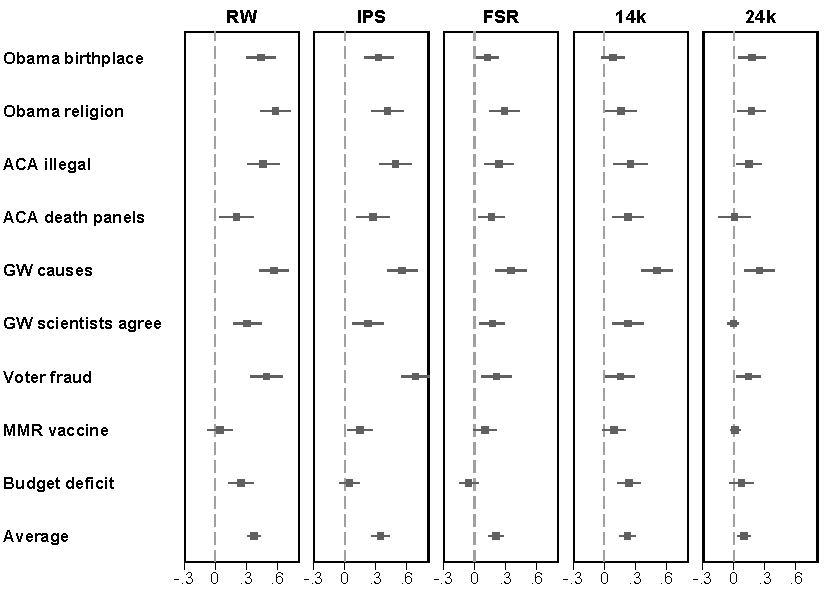
\includegraphics[scale=.8]{../figs/partisan-gap-by-item-arm.pdf}
		\label{fig:partisangaps-mturk}
		\caption*{\footnotesize 
			Each marker is the estimated gap between Republican partisans and Democratic partisans for how congenial their responses are to their own party.
			Columns indicate the five different treatment arms described in \nameref{sec:data}. Rows indicate the nine individual survey items described in \cref{si:mturk} plus their average.
			Horizontal bars are 95\% confidence intervals constructed from robust standard errors.
		}
	\end{figure}
\end{center}

We start by examining the average in partisan gaps for each survey item and each treatment arm. \Cref{fig:partisangaps-mturk} shows the results. Each marker represents how much more congenial the responses of the Republicans are to the Democrats.
In the RW treatment arm (first column), the Republicans are on average 0.3 percentage points more likely than the Democrats to have party-congenial responses. The subsequent four columns are in \cref{fig:partisangaps-mturk} show that while the estimated differences in party-congenial responses are precise (the narrow bars), the differences attenuated substantially depending on the treatment arms. This attenuation is most pronounced when comparing the RW to the 24k arms (first vs second columns).

We formalize the above observation as follows. We regress the dependent variable, which is an indicator for whether the response is party-congenial, on the interaction of partisanship and the treatment arm:
\begin{equation}\label{eq:partisangap-mturk}
	y_{ijk} = \alpha + \beta (Rep)_i + \gamma (Arm)_k + \delta_k (Rep_i \times Arm_k) + (survey \; item)_j + \varepsilon_{ijk}
\end{equation}
for respondent $i$, survey item $j$, and treatment arm $k$. $\beta$ is the difference in partisan knowledge gaps, which corresponds to \cref{fig:partisangaps-mturk}. A positive estimate suggests that Republicans are more likely than Democrats to have a party-congenial response.
We focus on the $\delta$'s, which capture how the different treatment arms affect observed partisan knowledge gaps. The baseline treatment arm is always RW, so that $\delta$ captures how the treatment arms---how the same question is phrased in different ways---mediates partisan knowledge gaps.
$(survey \; item)_j$ is the fixed effects for the nine survey items.
Standard errors are clustered at the respondent level.

\begin{figure}[!t]
	\centering
	\caption{Partisan Gap by Treatment Arm}
	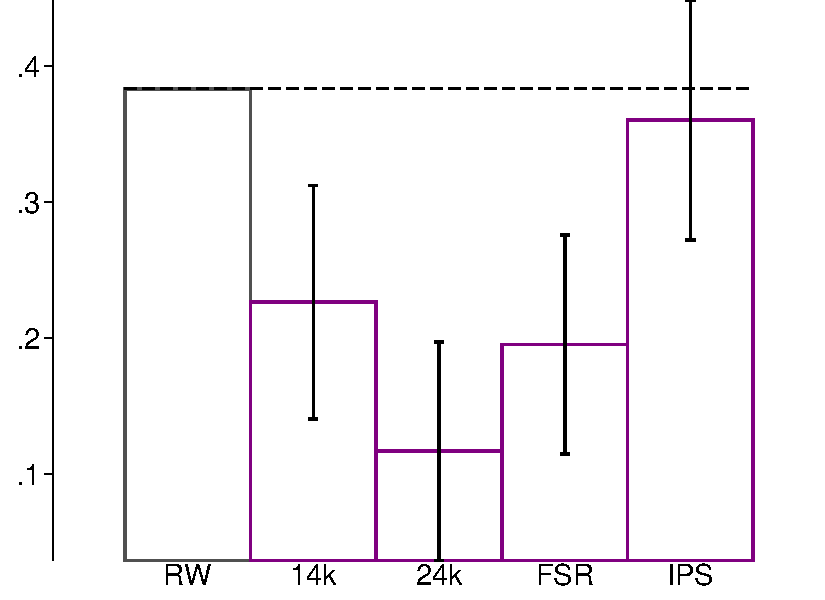
\includegraphics[scale=.6]{../figs/mturk-pgag-surveyarms.pdf}
	\label{fig:partisangaps-mturk-reg}
	\caption*{\footnotesize 
	Bars indicate the predicted partisan gap by the treatment arms. 
	Bars are reconstructed from the interactions of the Republican indicator with the treatment arms as reported in column (3) of \cref{tab:partisangaps-mturk}.
	Capped vertical bars are 95\% confidence intervals.
	}
\end{figure}
\cref{tab:partisangaps-mturk} reports the results from estimating \cref{eq:partisangap-mturk}. Column (1) includes just the Republican variable, which is significant and consistent with conventional wisdom about gaps in partisan knowledge \citep[e.g.][]{bullocketal_2015, pew2018disagree}.
Column (2) includes only the treatment arms, and three of them elicit differences in partisan gaps that are statistically different from the baseline RW arm. While the treatment arm estimates are not as large as the Republican variable in column (1), it is still substantial evidence of how variable the estimated knowledge gap can be.
Moreover, it is variable in a way that is orthogonal to partisanship. For instance, the average respondent assigned to the 24k arm is 17 percentage points less likely to give a party-congenial response than the RW arm ($p<0.001$). This gap is approximately two-thirds of the estimated effect of partisanship on the partisan knowledge gap.

In column (3) of \cref{tab:partisangaps-mturk}, we include the interaction of partisanship and treatment arms. Now the Republican variable captures the partisan gap in the RW arm (corresponding to column (1) of \cref{fig:baltest-24k-rw}). The republican and treatment arms interactions then tell us how the extent to which partisan knowledge gap changes across the different treatment arms. 

\cref{fig:partisangaps-mturk-reg} shows the estimates in absolute terms.
For the FSR interaction term, just adding a `Don't Know' response option reduces the estimated partisan knowledge gap by half ($p<0.001$).
The largest reduction comes from the 24k arm, which allows respondents to rate their responses on a 0 to 10 scale from `definitely false' to `definitely true' instead of a false and true option. Here, the estimated partisan knowledge gap reduction is 71 percent ($p<0.001$). Including self-reported characteristics of respondents in columns (4)--(6) does not change this conclusion. Estimated partisan knowledge gaps are highly variable to how the same question is posed to respondents.

\begin{table}[t] \centering \small \setlength\tabcolsep{0 pt} \setlength{\defaultaddspace}{0pt}
	\def\sym#1{\ifmmode^{#1}\else\(^{#1}\)\fi}
	\caption{Partisan Knowledge Gaps: MTurk}
	\label{tab:partisangaps-mturk}
	\begin{adjustbox}{max width=\textwidth}
		\begin{tabular}{l*{6}{D{.}{.}{-1}}}
			\toprule
			% https://tex.stackexchange.com/questions/567985/problems-with-inputtable-tex-hline-after-2020-fall-latex-release
			\input ../tabs/mturk-reg-table-fragment.tex
			\bottomrule
		\end{tabular}
	\end{adjustbox}
	\caption*{\footnotesize All models are linear probability models where the dependent variable indicates whether response to a survey item is congenial to party affiliation. Demographic controls include age cohort, gender, education level (college degree, high school, no high school, post-graduate, and some college), and race (Hispanic, Asian, Black, White, Others). All models include the nine survey item fixed effects. Standard errors are clustered at the respondent level. Significance levels: + 0.1 * 0.05 ** 0.01 *** 0.001.}
\end{table}

\subsection{Partisan Cues}\label{subsec:partisan-cues}
The aim of the study is to present experimental evidence about effect of partisan cues in the question stem on responses by partisans. For the purpose of the study, we examine closed-ended items asking about policy-relevant facts or objective performance, particularly those items stirring affective consistency, stereotyping, or both.  In the first case, items whose correct response option one side or the other would like to disbelieve, or at least one of whose incorrect response options one side or the other would like to believe, or both; in the second case items whose correct response option defies stereotype, or at least one of whose incorrect response options conforms to stereotype, or both.  

For exploring the research question, we exploit two datasets – a national survey conducted by YouGov, and a telephone survey of a random sample of adults in Texas and. The YouGov survey interviewed 2000 respondents between July 10th and 12th, 2012.  In Texas, a total of 1003 interviews were conducted between September 10th and 21st, 2012. 

In the YouGov survey, respondents were randomly assigned to factual questions with either a Republican or Democratic cue in the stem. In a question about whether ``since 2010 midterm elections, the unemployment rate [had] gone up, down, or remained the same, or couldn't you say?'', we inserted either the phrase “when Republicans regained control of the U.S. Congress'' or ``when Democrats retained control of the Senate” right after the first phrase. We employed a similar manipulation for the question on budget deficit, asking how the budget deficit had fared “since the 2010 midterm elections, when Republicans regained control of the U.S. Congress (or ``when Democrats retained control of the Senate''), has the budget deficit gone up, gone down, remained the same, or couldn't you say?''
In the Texas survey, we added another condition to the above design – no partisan cue in the stem. So a third of the respondents were assigned to a question that simply read, ``since the 2010 midterm elections, has the unemployment rate gone up, gone down, or remained the same?  Or couldn’t you say?'' For the second question we changed our design to – no partisan cue, Democratic cue, and Democratic cue plus the following introduction “based on what you have heard”. The question read, ``since January 2009, have federal taxes increased, decreased, or remained the same or couldn’t you say?.'' The second version gave respondents a Democratic cue by changing the initial part of the sentence; the question now read, “Since Barack Obama took office\ldots''  The third version prepended a cue designed to encourage guessing to the second version; the version read, “Based on what you have heard, since Barack Obama took office, \ldots''





\clearpage
\section*{Partisan Knowledge Gaps}
\begin{figure}[ht]
	\caption{Partisan Knowledge Gaps with Partisan Cues: YouGov Survey}	
	\centering
	\begin{subfigure}{.495\textwidth}\centering
		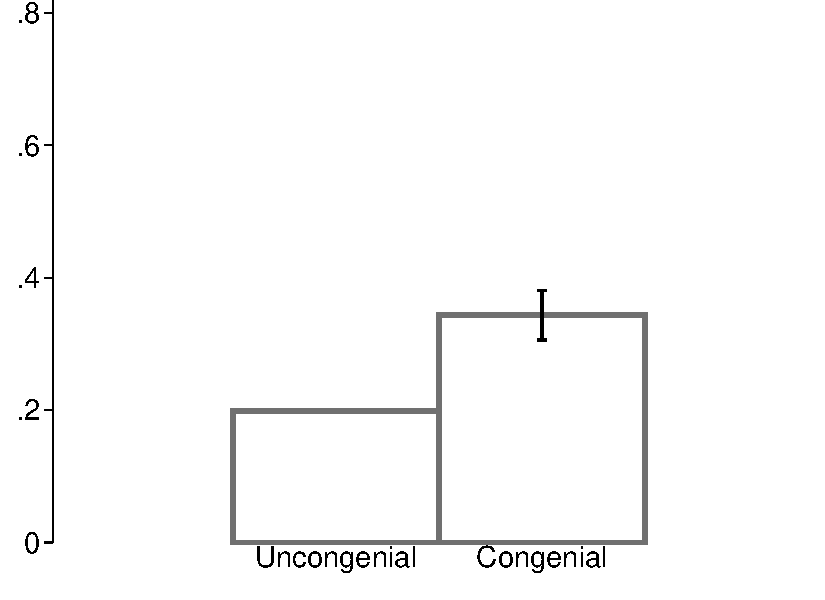
\includegraphics[width=\textwidth]{../figs/yougov-unemp-congenialcue.pdf}
		\caption{Unemployment}
	\end{subfigure}
	\hfil
	\begin{subfigure}{.495\textwidth}\centering
		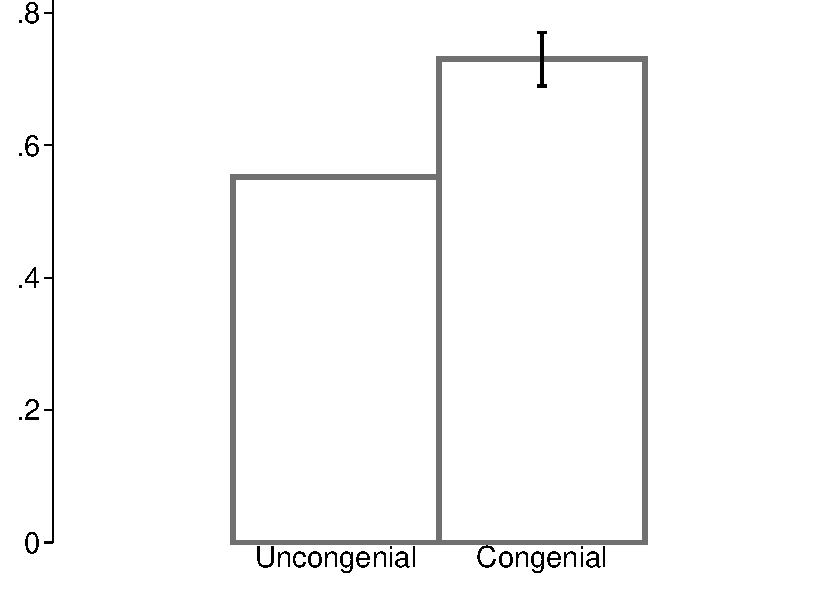
\includegraphics[width=\textwidth]{../figs/yougov-deficit-congenialcue.pdf}
		\caption{Budget deficit}
	\end{subfigure}	
	\caption*{\footnotesize Bars indicate the predicted percent of responses saying that unemployment or the budget deficit have gone up (correct responses) as reported in \cref{tab:partisangaps-yougov} (columns (1) and (4)).  
	Capped vertical bars indicate 95\% confidence intervals.
	}
	\label{fig:yougov-reg}
\end{figure}

We start with the YouGov survey to provide experimental evidence that cues in survey questions can affect responses to questions about policy-relevant and objectively verifiable facts. This survey includes questions about changes in unemployment and the budget deficit since the 2010 midterm elections, with manipulated partisan cues in the stem. 

Using the YouGov survey responses, we estimate
\begin{equation}\label{eq:pgap-yougov}
\text{correct response}_{i} = \alpha + \beta (congenial \; cue)_i  +\varepsilon_{i},
\end{equation}
where the dependent variable is the indicator for whether the response to the question is correct.
As discussed above in \cref{subsec:partisan-cues}, we model correct response rate as dependent on whether the cue presented to individuals is congenial to responding correctly.
Specifically, the congenial cue indicator is coded as one when a Democrat receives a question stem with the cue ``when Republicans gained control of the US congress.'' This cue manipulates Democrats into blaming the Republicans by suggesting that unemployment has gone up, which is the correct response.
The reverse happens for Republicans, where the congenial cue is coded as one when they receive the cue ``When Democrats retained control of the Senate.''

Panel (a) of \cref{fig:yougov-reg} shows that, by manipulating the partisan cue that respondents receive, the probability of getting the correct response for the unemployment question differs by 14 percentage points ($p < 0.001$, reported in \cref{tab:partisangaps-yougov}).

Panel (b) of \cref{fig:yougov-reg} shows that this systematic difference is not unique to the unemployment question. We reestimate \cref{eq:pgap-yougov} where the dependent variable is getting the correct response that the budget deficit has gone up. When the individuals get a congenial cue, they are 18 percentage points more likely to get the correct response ($p<0.001$).
Presumably, we observe this congenial cue effect because the question stem holds the other party responsible for the increase in unemployment and deficit, which are both undesirable.

\cref{fig:yougov-reg-by-partisanship} show that there is some heterogeneity in how the congenial cue affects Republicans as opposed to Democrats. However, the effect is not unique to either party since partisans of both types are more likely to get the correct response when randomly assigned the congenial cue.

\begin{table}[t] \centering \normalsize \setlength\tabcolsep{0 pt} \setlength{\defaultaddspace}{0pt}
	\def\sym#1{\ifmmode^{#1}\else\(^{#1}\)\fi}
	\caption{Partisan Knowledge Gaps with Partisan Cues: YouGov}
	\label{tab:partisangaps-yougov}
	\begin{adjustbox}{max width=\textwidth}
		\begin{tabular}{@{\hspace{0\tabcolsep}}l*{6}{D{.}{.}{-1}}@{\hspace{0\tabcolsep}}}
			\toprule
			% https://tex.stackexchange.com/questions/567985/problems-with-inputtable-tex-hline-after-2020-fall-latex-release
			&\multicolumn{3}{c}{Unemployment has gone up}&\multicolumn{3}{c}{Deficit has gone up}\\
			\cmidrule(lr){2-4}\cmidrule(l){5-7} 
			\input ../tabs/yougov-reg-table-fragment.tex
			\bottomrule
		\end{tabular}
	\end{adjustbox}
	\caption*{\footnotesize Dependent variables are indicators for whether the individual responded that unemployment or the budget deficit has gone up since the 2010 midterm elections (which are the correct responses).
	Congenial cue is an indicator for whether the question stem includes the cue towards getting the correct response. For Democrats, this is when the question stem includes the cue ``when Republicans gained control of the US Congress.''
	For Republicans, this is when the question stem includes the cue ``when Democrats retained control of the Senate.''
	Demographic controls include age cohort, gender, education level, marital status, employment status, news interest, family income, and race. Standard errors are heteroskedasticity-robust. 
	All models are linear probability models. 
	Significance levels: + 0.1 * 0.05 ** 0.01 *** 0.001.}
\end{table}

\clearpage
We further supplement our results with the Texas Lyceum survey, which affords a neutral cue. In this survey, in addition to congenial and uncongenial cues, individuals can also be randomly assigned a neutral cue where the additional question stem assigning blame to a party is absent, giving us a total of three groups: (i) no cue, (ii) congenial cue, and (iii) uncongenial cue.


\clearpage
\section*{Discussion and Conclusion}

Our results clarify our understanding of partisan knowledge gaps in important ways. First, partisan knowledge gaps are less ubiquitous than what conventional wisdom in political science suggests. For three in ten items, partisans either know \textit{less} party-congenial information or \textit{more} party-\textit{un}congenial information than their opponents. Among gaps occurring in the correct direction, we can only be certain that Democrats and Republicans actually differ from one another in their factual understanding of politics less than half the time. Secondly, the average knowledge gap in our data is small, with a mean gap of six percentage points and a median gap of about three percentage points. Third, many question features like the number of response options or question wording weakly predict the size of partisan knowledge gaps; instead, it is question difficulty and the \textit{content} of response options that influence the size of the gap.

If partisan gaps are small on average and difficult to predict based on question wording, why does the common wisdom that Democrats and Republicans differ substantially in political knowledge persist? One explanation may be that the knowledge items in our dataset are a not a representative set of relevant cognitions that partisans have. It may well be that the knowledge gaps are larger on partisan-relevant facts that are not asked about in the studies described above. To what degree this is so, we cannot say, except to note that the general bias is to ``hunt where the ducks are.'' That is, in at least two of our studies \citep{bullocketal_2015, prior2015you}, expert political scientists constructed knowledge questions that they reasonably believed \textit{a priori} would produce large partisan gaps; in the case of \citet{jerit2012partisan}, the authors built a dataset of knowledge questions that they believed carried a partisan implication (in other words, in which they expected knowledge gaps between Democrats and Republicans to occur). The fact that statistically significant, ``positive'' knowledge gaps only emerge on about half of the items from these studies suggests that partisan knowledge gaps are less common even when looking in the most obvious place. 

A potentially more satisfying explanation for this discrepancy is that such conventional wisdom is largely based on studies using data from the \citet{anes_gen}. Much of the literature on partisan knowledge gaps has built upon \citet{bartels_2002}, who was the first to write about these differences \citep{bullocklenz_2019}. For example, using the ANES data, \citet{bartels_2002} discovered that Democrats and Republicans reported different beliefs on a variety of objective facts---such as how inflation and unemployment changed over the previous eight years---while Ronald Reagan was president. In 1988, the estimated differences between Democrats and Republicans on knowledge questions ranged from approximately 12 to 36 percentage points, depending on the question.\footnote{These figures have been rescaled in percentage point terms. \citeapos{bartels_2002}  original calculation is that ``the estimated differences between Democrats and Republicans rang[e] from .249 to .715 on the -1 to +1 scales'' (137).} These kinds of questions with imprecise response options---which ask about respondents' \textit{assessment} of politically relevant facts rather than their actual \textit{knowledge} of such facts---are one of the most likely source of large partisan knowledge gaps. The fact that questions with imprecise response options are commonplace on one of the biggest publicly-available sources of survey data likely helps perpetuate the idea that Democrats and Republicans approach the political world with entirely different information. 

Based on our results here, we suspect that the vast majority of partisan gaps---when they do appear---are more likely to be a product of motivated responding than of partisans simply knowing different things (\citeauthor{bisgaard_slothuus_2018} \citeyear{bisgaard_slothuus_2018}; \citeauthor {bullocketal_2015} \citeyear{bullocketal_2015}; \citeauthor{prior2015you} \citeyear{prior2015you}; \citeauthor{schaffner_luks} \citeyear{schaffner_luks}; but see \citeauthor{berinsky_2017} \citeyear{berinsky_2017} and \citeauthor{peterson_iyengar_forth} \citeyear{peterson_iyengar_forth}). None of this is to say that partisan bias does not play a role in shaping how Democrats and Republicans interpret what they know; there is ample evidence to suggest that it does \citep[e.g.,][]{bisgaard2015bias, gainesetal_2007, khanna2018motivated}. Nor should the small size of the average gap prevent us from noting that on many of the questions, a majority of partisans on both sides of the aisle were either ignorant or misinformed about the facts: the average proportion of Republicans and Democrats who provided correct answers to these knowledge questions is about 42\% each. 

While this is certainly troubling for those who view political knowledge as an essential component of democratic citizenship, there is some reason for optimism. When it comes to knowledge of political facts, more often than not, there do not appear to be large imbalances between what Democrats and Republicans know. When partisan differences do emerge, we suspect that they are often more a product of biased interpretation of survey questions rather than of differential stores of knowledge. This suggests that even in a polarized political context, most Democrats and Republicans can use the same information to make collective judgments about whether to reward or punish elected officials based on performance---whether they want to, of course, is another question. 



\clearpage
\bibliographystyle{apsr}
\bibliography{pgap}

\clearpage

\appendix
\renewcommand{\thesection}{SI \arabic{section}}
\setcounter{table}{0}\renewcommand\thetable{\thesection.\arabic{table}}  
\setcounter{figure}{0}\renewcommand\thefigure{\thesection.\arabic{figure}}
\counterwithin{figure}{section}


\begin{center}
\Large \textbf{SUPPORTING INFORMATION}
\end{center}
\singlespacing
\vspace{-.4in}

\section{Supporting figures}
\begin{center}
\begin{figure}[H]
  \centering
  \caption{Balance test: MTurk}
  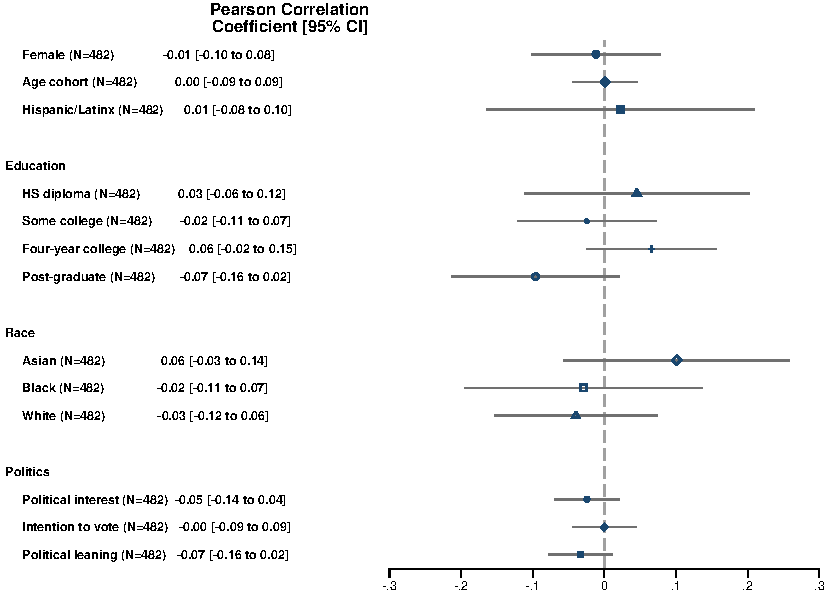
\includegraphics[scale=.8]{../figs/baltest-24k-rw.pdf}
  \label{fig:baltest-24k-rw}
  \caption*{\footnotesize Figure shows the results from a balance test for the Amazon Mechanical Turk sample. Self-reported characteristics of respondents are compared between the respondents assigned to the 24k arm and the RW arm as described in \nameref{sec:data}. 
  Rows are self-reported characteristics.
  Second column reports the correlation between characteristics and the 24k arm, and the 95\% confidence intervals constructed from bootstrapped standard errors (n=10,000).
  Third column reports the estimated difference between the 24k respondents and the RW respondents.
  Horizontal bars are 95\% confidence intervals constructed from robust standard errors.
  }
\end{figure}
\end{center}


\begin{figure}[ht]
	\caption{Partisan Knowledge Gaps with Partisan Cues: YouGov}	
	\centering
	\begin{subfigure}{.495\textwidth}\centering
		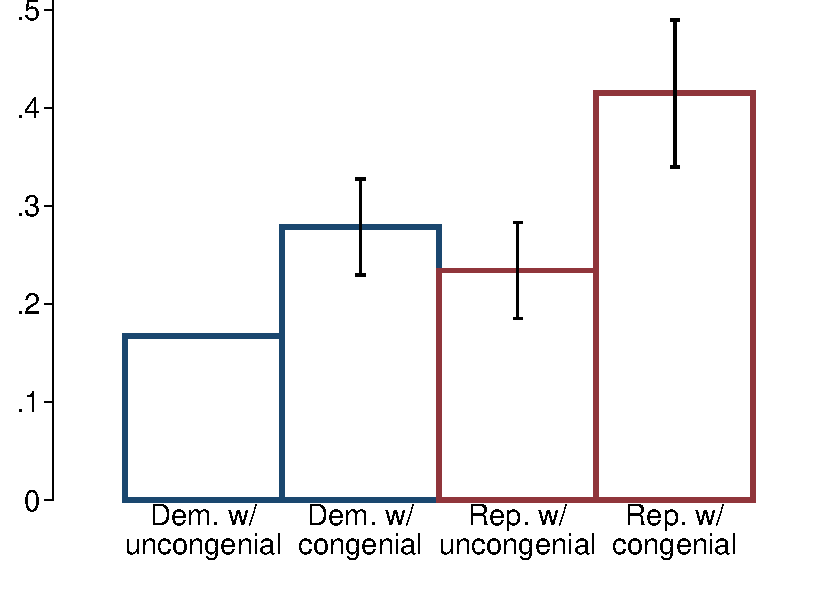
\includegraphics[width=\textwidth]{../figs/yougov-unemp-congenialcue-partisan.pdf}
		\caption{Unemployment}
	\end{subfigure}
	\hfil
	\begin{subfigure}{.495\textwidth}\centering
		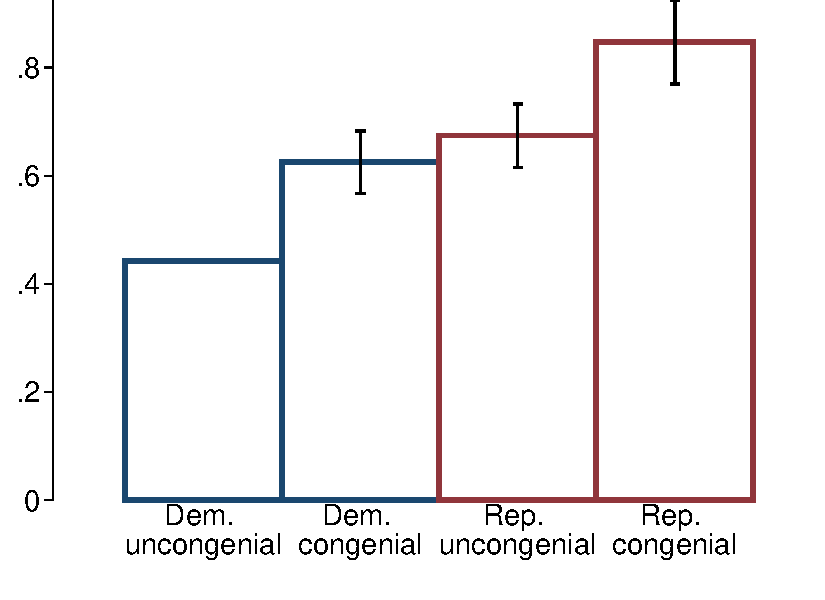
\includegraphics[width=\textwidth]{../figs/yougov-deficit-congenialcue-partisan.pdf}
		\caption{Budget deficit}
	\end{subfigure}	
	\caption*{\footnotesize Figure shows the effect of congenial cues for the YouGov survey by partisanship. Bars indicate the predicted percent of responses saying that unemployment have gone up (correct response) as retrieved from the estimates in \cref{tab:partisangaps-yougov} (columns (2) and (5)).  The estimates are obtained by estimating:\\
		
	$\qquad\text{correct response}_{i} = \alpha + \beta (congenial \; cue)_i + \gamma (Rep)_i + \delta (congenial\; cue \times Rep)_i + \varepsilon_{i}$.\\
	
	Capped vertical bars indicate 95\% confidence intervals.
	}
	\label{fig:yougov-reg-by-partisanship}
\end{figure}

\clearpage
\section{Item Text for the MTurk Study}\label{si:mturk}

\textbf{Preface for Different Conditions}

\textbf{RW, IP}\newline
Now here are some questions about what you may know about politics and public affairs.

\textbf{FSR, 14k, 24k}\newline
Now here are some questions about what you may know about politics and public affairs.
We are interested in measuring what people currently know and can recall on their own and are
just as interested in what people don't know as in what they do know. So we'd like your
agreement to just say ``don't know'' if you don't know the answer—without looking anything up
or talking with anyone about it.

\textbf{Item Text}
\textbf{24k}\newline
Now here are a series of statements. On a scale of 0 to 10, where 0 means definitely false,
10 means definitely true, and 5 is exactly in the middle, how definitely true or false is
each statement?

\begin{itemize}
	\item Barack Obama was born in the US (T)
	\item  Barack Obama is a Muslim (F)
	\item  The Affordable Care Act gives illegal immigrants financial help to buy health insurance (F)
	\item  The Affordable Care Act does not create government panels to make decisions about end-of-life care (T)
	\item  Temperatures around the world are increasing because of human activity, like burning coal and gasoline (T)
	\item  Most climate scientists believe that global warming is not occurring (F)
	\item  In the 2016 presidential election, President Trump won the majority of the legally cast votes (F)
	\item  The vaccine for measles, mumps, and rubella (MMR) causes autism in children. (F)
	\item  Since 2012, the annual federal budget deficit has increased. (T)
\end{itemize}

\textbf{Rest of the Conditions, By Item}

\begin{itemize}
\item Obama's Birthplace

\textbf{RW and IP}\newline

According to the Constitution, American presidents must be ``natural born citizens.''
Some people believe Barack Obama was not born in the United States, but was born
in another country. Do you think Barack Obama was born in ...?
\begin{itemize}
	\item The US
	\item Another country
\end{itemize}

\textbf{FSR}\newline
Some people believe Barack Obama was not born in the United States, but was born
in another country. Was he born in ...?
\begin{itemize}
	\item The US
	\item Another country
	\item DK (plus DK pref)
\end{itemize}

\textbf{14k}\newline

Was Barack Obama born in ...?
\begin{itemize}
	\item the US
	\item Another country
	\item DK (plus DK pref)
\end{itemize}

\item Obama Religion\newline
\textbf{RW}\newline

Do you personally believe that Barack Obama is a ...?
\begin{itemize}
	\item Muslim
	\item Christian
\end{itemize}

\textbf{IP}\newline

Most people have a religion. Some people believe Barack Obama is a Muslim. Do
you personally believe that Barack Obama is a \ldots?
\begin{itemize}
	\item Muslim
	\item Christian
\end{itemize}

\textbf{FSR}\newline

Some people believe Barack Obama is a Muslim. Is he a \ldots?
\begin{itemize}
	\item Muslim
	\item Christian
	\item DK (+ DK pref)
\end{itemize}

\textbf{14k}\newline

Is Barack Obama a \ldots? 
\begin{itemize}
	\item Muslim
	\item Christian
	\item DK (plus DK pref)
\end{itemize}

\item ACA Illegal\newline
\textbf{RW}\newline

To the best of your knowledge, would you say the Affordable Care Act\ldots?
\begin{itemize}
	\item Gives illegal immigrants financial help to buy health insurance
	\item Does not give illegal immigrants financial help to buy health insurance
\end{itemize}

\textbf{IP}\newline

As you may know, there is currently talk of changing the Affordable Care Act
(ACA), enacted in 2010. Some people believe that the ACA gives illegal immigrants
financial help to buy health insurance. To the best of your knowledge, would you say
the ACA\ldots?
\begin{itemize}
	\item Gives illegal immigrants financial help to buy health insurance
	\item Does not give illegal immigrants financial help to buy health insurance
\end{itemize}

\textbf{FSR}\newline

Some people believe that Affordable Care Act gives illegal immigrants financial help
to buy health insurance. Does the Affordable Care Act\ldots?
\begin{itemize}
	\item Give illegal immigrants financial help to buy health insurance
	\item Not give illegal immigrants financial help to buy health insurance
	\item DK (+ DK pref)
\end{itemize}

\textbf{14k}\newline
Does the Affordable Care Act\ldots?
\begin{itemize}
	\item Give illegal immigrants financial help to buy health insurance
	\item Not Give illegal immigrants financial help to buy health insurance
	\item Don't know (+ DK pref)
\end{itemize}

\item ACA—Death Panels\newline
\textbf{RW}\newline
To the best of your knowledge, would you say that the Affordable Care Act \ldots?
\begin{itemize}
	\item Creates government panels to make decisions about end-of-life care
	\item Does not create government panels to make decisions about end-of-life care
\end{itemize}

\textbf{IP}\newline 

Some people believe that Affordable Care Act establishes a government panel to
make decisions about end-of-life care. To the best of your knowledge, would you say
that the Affordable Care Act \ldots?
\begin{itemize}
	\item Creates government panels to make decisions about end-of-life care
	\item Does not create government panels to make decisions about end-of-life care
\end{itemize}

\textbf{FSR}\newline

Some people believe that Affordable Care Act establishes a government panel to
make decisions about end-of-life care. Does the Affordable Care Act\ldots?
\begin{itemize}
	\item Creates government panels to make decisions about end-of-life care
	\item Does not create government panels to make decisions about end-of-life care
	\item DK (+ DK pref)
\end{itemize}

\textbf{14k}\newline
Does the Affordable Care Act \ldots?
\begin{itemize}
	\item Creates government panels to make decisions about end-of-life care
	\item Does not create government panels to make decisions about end-of-life care
	\item DK (+ DK pref)
\end{itemize}

\item Global Warming—Happening + Causes\newline
\textbf{RW}\newline
Which of the following best fits your view about this? Are temperatures around the
world \ldots?
\begin{itemize}
	\item Increasing because of natural variation over time, such as produced the ice age
	\item Increasing because of human activity, like burning coal and gasoline
	\item Staying about the same as they have been
\end{itemize}

\textbf{IP}\newline
Recently, you may have noticed that global warming has been getting some attention
in the news. Some people believe that temperatures are increasing around the world
because of natural variation over time, such as produced the ice age. Which of the
following best fits your view about this? Would you say that temperatures around the
world are\ldots?
\begin{itemize}
	\item Increasing because of natural variation over time, such as produced the ice age
	\item Increasing because of human activity, like burning coal and gasoline
	\item Staying about the same as they have been
\end{itemize}

\textbf{FSR}\newline 

Some people believe that temperatures are increasing around the world because of
natural variation over time, such as produced the ice age. Are temperatures around
the world \ldots?
\begin{itemize}
	\item Increasing because of natural variation over time, such as produced the ice age
	\item Increasing because of human activity, like burning coal and gasoline
	\item Staying about the same as they have been
	\item DK (+ DK pref)
\end{itemize}

\textbf{14k}\newline
Are temperatures around the world \ldots?
\begin{itemize}
	\item Increasing because natural variation over time, such as produced the ice age
	\item Increasing because human activity, like burning coal and gasoline
	\item Staying about the same as they have been
	\item DK (+ DK pref)
\end{itemize}

\item GW—Scientist Agreement\newline
\textbf{RW}\newline
Just your impression, which one of the following statements do you think is most
accurate?
\begin{itemize}
	\item Most climate scientists believe that global warming is occurring.
	\item Most climate scientists believe that global warming is not occurring.
	\item Climate scientists are about equally divided about whether global warming is occurring or not
\end{itemize}

\textbf{IP}\newline
As you may know, the term ``global warming'' refers to the claim that temperatures
have been increasing around the world. Some people believe that most climate
scientists believe that global warming is not occurring. Just your impression, which
one of the following statements do you think is most accurate?
\begin{itemize}
	\item Most climate scientists believe that global warming is occurring.
	\item Most climate scientists believe that global warming is not occurring.
	\item Climate scientists are about equally divided about whether global warming is occurring or not
\end{itemize}
\textbf{FSR}\newline
Some people believe that most climate scientists believe that global warming is not
occurring. Which one of the following statements is most accurate?
\begin{itemize}
	\item Most climate scientists believe that global warming is occurring.
	\item Most climate scientists believe that global warming is not occurring.
	\item Climate scientists are about equally divided about whether global warming is occurring or not 
	\item DK (+ DK pref)
\end{itemize}

\textbf{14k}\newline
Which one of the following statements is most accurate?
\begin{itemize}
	\item Most climate scientists believe that global warming is occurring.
	\item Most climate scientists believe that global warming is NOT occurring.
	\item Climate scientists are about equally divided about whether global warming is occurring or not
	\item DK (+ DK pref)
\end{itemize}

\item Voter Fraud\newline
\textbf{RW}\newline
As you may know, President Trump has said that several million people voted
illegally in the 2016 presidential election and that he won the majority of the legally
cast votes. Do you believe that President Trump \ldots?
\begin{itemize}
	\item Won the majority of the legally cast votes
	\item Did not win the majority of the legally cast votes
\end{itemize}

\textbf{IP}\newline
As you may know, not everyone living in the US has the legal right to vote. President
Trump has said that several million people voted illegally in the 2016 presidential
election and that he won the majority of the legally cast votes. Do think that that
President Trump \ldots?
\begin{itemize}
	\item Won the majority of the legally cast votes
	\item Did not win the majority of the legally cast votes
\end{itemize}

\textbf{FSR}\newline
As you may know, President Trump has said that several million people voted
illegally in the 2016 presidential election and that he won the majority of the legally
cast votes. Did President Trump \ldots?
\begin{itemize}
	\item Won the majority of the legally cast votes
	\item Did not win the majority of the legally cast votes
	\item DK (+ DK pref)
\end{itemize}

\textbf{14k}\newline
In the 2016 presidential election, did President Trump \ldots?
\begin{itemize}
	\item Won the majority of the legally cast votes
	\item Did not win the majority of the legally cast votes
	\item DK (+ DK pref) 
\end{itemize}

\item Vaccines\newline
\textbf{RW}\newline
From what you have read or heard, do you personally think that the vaccine for
Measles, Mumps, and Rubella (MMR):
\begin{itemize}
	\item Causes autism in children
	\item Does not cause autism is children
\end{itemize}

\textbf{IP}\newline
As you may know, most children receive the vaccine for Measles, Mumps, and
Rubella (MMR). Some people believe that the MMR vaccine causes autism in
children. From what you have read or heard, do you personally think that the MMR
vaccine:
\begin{itemize}
	\item Causes autism in children
	\item Does not cause autism is children
\end{itemize}

\textbf{FSR}\newline
Some people believe that the vaccine for Measles, Mumps, and Rubella (MMR)
causes autism in children. Does the MMR vaccine \ldots?
\begin{itemize}
	\item Cause autism in children
	\item Not cause autism in children.
	\item DK (+ DK pref)
\end{itemize}

\textbf{14k}\newline
Does the vaccine for Measles, Mumps, and Rubella (MMR) \ldots?
\begin{itemize}
	\item Cause autism in children
	\item Not cause autism in children.
	\item DK (+ DK pref)
\end{itemize}

\item Obama—Budget Deficit\newline
\textbf{RW}\newline
As you may know, the federal government runs a deficit when it spends more than it
takes in. Since 2012, would you say that the annual federal budget deficit has \ldots
\begin{itemize}
	\item Increased
	\item Stayed about the same
	\item Decreased
\end{itemize}

\textbf{IP}\newline 
As you may know, the federal government runs a deficit when it spends more than it
takes in. Since 2012, with the Republicans having the majority in the U.S. House of
Representatives, would you say that the annual federal budget deficit has \ldots
\begin{itemize}
	\item Increased
	\item Stayed about the same
	\item Decreased
\end{itemize}

\textbf{FSR}\newline
Since 2012, with the Republicans having the majority in the U.S. House of
Representatives,
\begin{itemize}
	\item has the annual federal budget deficit \ldots.
	\item Increased
	\item Stayed about the same
	\item Decreased
	\item DK (+ DK pref)
\end{itemize}

\textbf{14k}\newline

Since 2012, has the annual federal budget deficit \ldots
\begin{itemize}
	\item Increased
	\item Stayed about the same
	\item Decreased
	\item DK (+ DK pref) 
\end{itemize}
\end{itemize}
\end{document}